\chapter{Introduction et contexte} \label{chap:1}
Ce premier chapitre présente l’équipe d’accueil ainsi que le contexte général de l’étude. Une présentation du parc électro-nucléaire français est faite. Une mise en contexte sur les accidents graves et la rétention du corium en cuve est ensuite présentée. Pour conclure un historique des travaux en lien avec le stage ainsi que l’objectif du stage sont exposés.
\section{Présentation du CEA et du laboratoire d'accueil}
Le Commissariat à l'Énergie atomique et aux énergies alternatives (CEA) est un organisme de recherche au service de l'État et des industriels divisé en quatre directions assurant des missions distinctes :
\begin{itemize}
	\item[$\bullet$] Direction des Applications Militaires (DAM) : mène des travaux sur l'ensemble du cycle de vie des armes nucléaires (conception, fabrication, entretien, démantèlement) ainsi que sur les chaufferies nucléaires des bâtiments de la marine nationale.
	\item[$\bullet$] Direction de Recherche Technologique (DRT) : dont la mission principale est le développement et le transfert de technologies de pointe vers des industriels locaux.
	\item[$\bullet$] Direction de la Recherche Fondamentale (DRF) : conduit des recherches dans des domaines très variés tels que les sciences de l'univers, la biotechnologie ou la fusion nucléaire.
	\item[$\bullet$] Direction des ÉnergieS (DES) : apporte une expertise sur l'ensemble des systèmes de production d'énergie, principalement le nucléaire sur l'ensemble du cycle de vie, de la conception au démantèlement et le traitement des déchets. 
\end{itemize}
Le laboratoire d'accueil est le Laboratoire de Modélisation des Accidents Graves (LMAG) du Département de Technologie Nucléaire (DTN) rattaché à l'Institut de REcherche sur les Systèmes Nucléaires pour la production d’Energie bas carbone (IRESNE) affilié à la Direction des ÉnergieS (DES) sur le centre de Cadarache.
Les travaux du laboratoire portent sur le comportement du c\oe ur fondu, que l'on nomme corium, en situation accidentelle. Les principaux axes de recherche du laboratoire se répartissent ainsi :
\begin{itemize}
	\item[$\bullet$] pour les réacteurs à neutrons rapides refroidis au sodium (RNR-Na), la propagation de l'accident depuis la dégradation du c\oe ur jusqu'à la stabilisation du corium sur un récupérateur est étudiée avec un intérêt particulier pour l'interaction corium-sodium ; 
	\item[$\bullet$] concernant les réacteurs à eau légère, ce sont les phases avancées qui sont étudiées : la comportement du corium en fond de cuve, l'étalement du corium hors cuve et son interaction avec le béton.
\end{itemize}
Ce laboratoire emploie quinze ingénieurs-chercheurs et quatre doctorants qui travaillent principalement sur la modélisation et la simulation numérique, étant ainsi complémentaire au Laboratoire d'Expérimentation des Accidents Graves (LEAG) qui exploite une plateforme expérimentale (PLINIUS) dédiée au corium prototypique. Le stage a été encadré par Mirantsoa-Aimé Rasolofomanana, doctorant et Romain Le Tellier, ingénieur-chercheur.

\section{Contexte de l'étude}
\subsection{Contexte industriel}
En France, 56 réacteurs nucléaires dispersés sur 18 sites sont actuellement en service. Ce parc est uniquement composé de réacteurs à eau pressurisée (REP) et représente 70\% de la production électrique française. Les puissances fournies par ces réacteurs dit de deuxième génération varient entre 900 MWe et 1450 MWe. Un réacteur de troisième génération d'une puissance de 1650 MWe (EPR - Evolutionary pressurized reactor) est actuellement en construction sur le site de Flamanville. Cette nouvelle génération de réacteur tient compte du retour d'expérience issu de l'exploitation des réacteurs actuels, intégrant notamment plus d'éléments de sûreté. La construction de six nouveaux EPR a été annoncée et huit autres pourraient voir le jour \cite{noauthor_emmanuel_2021}. \\
Les REP sont des réacteurs de la famille des réacteurs à eau légère, de l'eau ordinaire (H$_2$O) est utilisée comme fluide caloporteur et modérateur, de plus cette eau est pressurisée pour éviter un changement de phase liquide-gaz dans le circuit primaire et éviter tout risque d'asséchement, le schéma de principe de fonctionnement est présenté par la Figure \ref{fig:schcentrale1}. %, à l'entrée de la cuve la température de l'eau est 290\textdegree C et la température de sortie de cuve en fonctionnement nominal est de 330\textdegree C.
\begin{figure}[H]
	\centering
	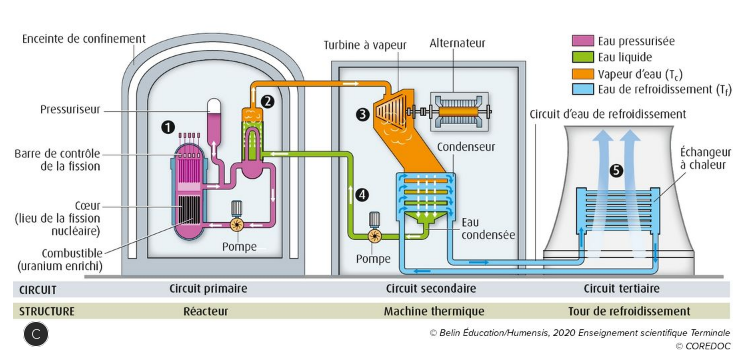
\includegraphics[width=0.9\linewidth]{figure/sch_centrale1}
	\caption[Schéma de principe d'une centrale nucléaire de type REP]{Schéma de principe d'une centrale nucléaire de type REP, d'après \cite{noauthor_manuel_nodate}}
	\label{fig:schcentrale1}
\end{figure} 
\subsection{Généralités sur la sûreté nucléaire}

Les questions relatives à la sûreté sont intrinsèquement liées à l'exploitation d'une centrale nucléaire tant les conséquences d'un éventuel accident peuvent être importantes. Ainsi dès le début des années 1970, le concept de défense en profondeur a été mis en place. ce dernier se matérialise par la mise en place de lignes de défense successives indépendantes. Les REP comptent trois barrières de confinement :
\begin{enumerate}
	\item la gaine combustible, constituée de zircaloy (alliage de zirconium) qui piège les produits radioactifs et notamment les gaz de fission dans les pastilles de combustibles ;
	\item la cuve et l'ensemble du circuit primaire ;
	\item le bâtiment réacteur placé sous atmosphère dépressurisée, dernière barrière de confinement avant la contamination hors-site.
\end{enumerate}
Les variations par rapport au régime nominal sont classées selon l'échelle INES (International Nuclear Scale Event, figure \ref{fig:echelle-ines-article}), cette échelle permet de classifier les accidents selon les conséquences engendrées. Elle comporte huit échelons allant d'un simple écart (plusieurs centaines de cas par an en France) à l'accident majeur entraînant une contamination hors site. Les accidents correspondent aux paliers 4 à 7 et se différencient de l'incident du fait de la perte d'intégrité de la première barrière à la suite d'une fusion du combustible pour former un bain liquide issu du c\oe ur fondu : le corium.
\begin{figure}[H]
	\centering
	%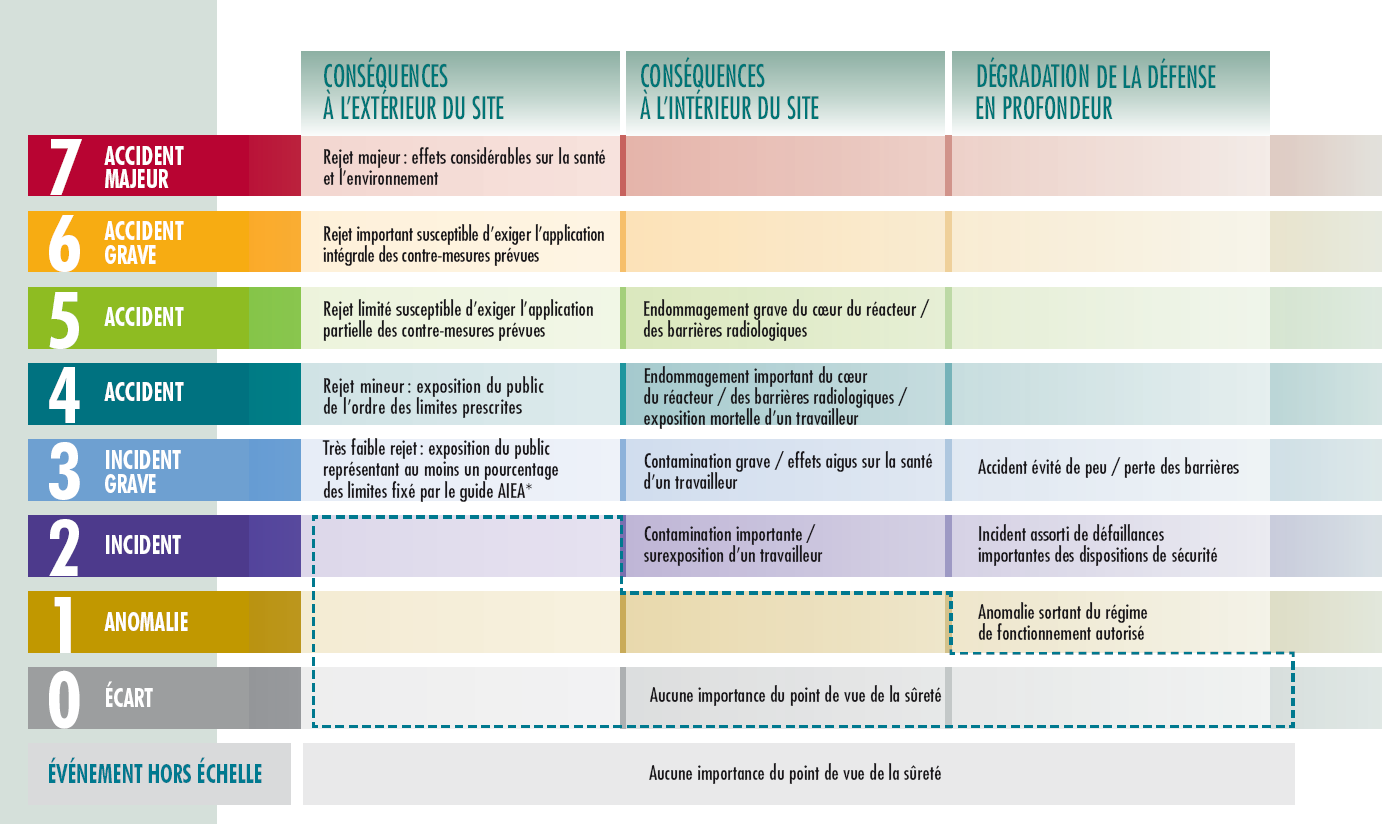
\includegraphics[width=1\linewidth]{figure/echelle-ines-article}
	\includegraphics[width=1\linewidth]{figure/RTN_ines}
	\caption[Echelle de classification des écarts au régime nominal INES]{Echelle de classification des écarts au régime nominal INES, d'après \cite{noauthor_risque_nodate}}
	\label{fig:echelle-ines-article}
\end{figure}
Les accidents possibles dans les REP sont séparés en deux grandes catégories : les accidents de criticité et les Accidents de Perte de Réfrigérant Primaire (APRP). Les accidents de criticité sont dus à une accélération brutale de la réaction en chaîne, le c\oe ur est alors en régime sur-critique ce qui entraîne une augmentation rapide de puissance thermique produite. L'accident de Tchernobyl en 1986, survenu sur un réacteur d'une technologie différente de celle des REP, est un exemple d'accident de criticité.\\ Les Accidents de Perte de Réfrigérant Primaire (APRP) résultent quant à eux d'une fuite dans le circuit primaire ou d'un arrêt de la circulation du fluide caloporteur privant le c\oe ur du refroidissement nécessaire à son fonctionnement, un cas d'accident de ce type est Fukushima Daiichi en 2011 où le tsunami a provoqué la perte d'alimentation électrique de la centrale, neutralisant ainsi l'ensemble des pompes. \\
Lors d'un accident de type APRP, l'élévation de la température dans le c\oe ur provoque l'oxydation fortement exothermique des gaines en zircaloy. La puissance produite par cette oxydation peut être, transitoirement,  supérieure à la puissance résiduelle liée à la désintégration naturelle des radioéléments. Sans refroidissement suffisant l'augmentation de température provoque la fusion du combustible, puis des éléments de contrôle du c\oe ur. Finalement le mélange issu de la fusion du combustible, des gaines partiellement oxydées et des structures internes du réacteur forme un bain liquide appelé corium. Le corium est un matériau fortement radioactif produisant sa propre chaleur, il est constitué d'uranium U, d'oxygène O, de zirconium Zr sous st\oe chiométrique ainsi que d'acier issu des structures.  L'objectif est alors de maîtriser la propagation de ce liquide, pour cela deux stratégies existent : la rétention en fond de cuve avec refroidissement externe, \textit{In-Vessel Retention, IVR} \cites{shi_cap1400_2019}{seiler_etudes_2010}. Pour limiter les conséquences d'un accident cette stratégie vise à maintenir le corium au fond de la cuve réacteur. Pour cela un refroidissement à l'extérieur de la cuve est mis en place. Cette stratégie est étudiée depuis les années 90 et mise en \oe uvre sur des réacteurs de faible puissance.
Une seconde stratégie, préférée pour les réacteurs de forte puissance, consiste à étaler le corium sur un radier en béton réfractaire \cite{bouteille_epr_2006}. Dans le cas de l'EPR, l'ablation du béton est limitée par un refroidissement passif mis en place sous le plancher, une fois le corium partiellement refroidi, celui-ci est finalement recouvert d'eau évitant ainsi une explosion de vapeur.\\
Dans la suite de ce rapport nous traiterons uniquement les cas d'accidents de type APRP et de rétention du corium en cuve \textit{IVR}.
\subsection{Stratégie de rétention du corium en fond de cuve (IVR)}
Le comportement du corium en fond de cuve est alors régi par deux principaux phénomènes \cite{shams_status_2020} : 
la thermochimie détermine le comportement des phases et leurs équilibres, en effet la présence d'une lacune de miscibilité pour la phase liquide du système \{U, O, Zr, Acier\} entraîne une stratification des phases liquides. En effet on distingue alors plusieurs phases dans le bain, une phase oxyde riche en oxygène et une ou plusieurs phases pauvre en oxygène notées métal. Le second phénomène concerne la thermohydraulique du bain, chaque phase est soumise à des mouvements de convection naturelle induite par les conditions aux limites associées (instabilité de Rayleigh-Bénard) et/ou le chauffage volumique associée à la puissance résiduelle.
%\subsubsection{Modélisation stationnaire}
Les premières études du comportement du bain de corium ont été réalisés pour des bains stationnaires. Il a été montré qu'en régime stationnaire la stratification comprend une phase oxyde et une phase métal \cite{theofanous_-vessel_1997}, cependant en fonction de l'accident la couche de métal peut être lourde (i.e plus que l'oxyde, on retrouve alors la configuration \ref{fig:confmetallourd}) ou légère (configuration \ref{fig:confmetalleger}). Les différents cas sont obtenus via des différences de conditions initiales (fraction massique d'acier, degré d'oxydation du zirconium, le rapport molaire entre l'uranium et le zirconium dans la phase oxyde et la température du bain). On distingue également, à certaines interfaces entre la cuve et le bain, la présence d'une croûte réfractaire issue de la solidification de la phase oxyde.
\begin{figure}[H]
	\begin{subfigure}[H]{0.47\textwidth}
		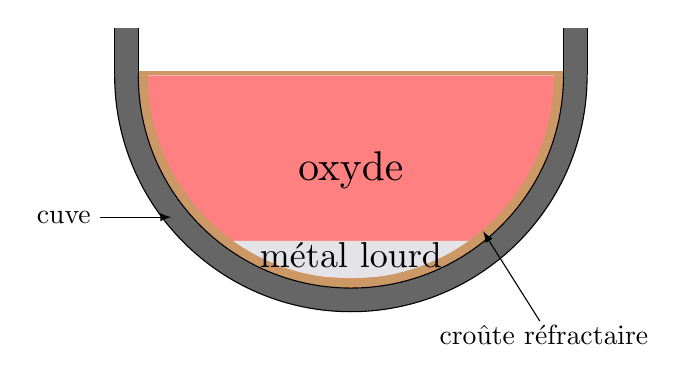
\begin{tikzpicture}[scale=0.60]
		%cuve
		%couche+croute
		\fill[red!50] (0.5,0) arc (180:360:4.5) -- cycle;
		%\fill[blue!10!gray!20] rectangle (9.5, 1);
		\fill[brown!80] (0.5,0) arc (180:360:4.5) -- (9.3,0) arc (360:180:4.3) -- cycle;
		\fill[brown!80] rectangle (9.5,0.1);
		\fill[blue!10!gray!20] (2.5,-3.5) ..controls +(0.9,-1.05)and+(-0.9,-1.05) .. (7.5,-3.5) -- cycle ;
	\fill[black!60] (0,1) -- (0,0) arc (180:360:5) -- (10,1) -- (9.5,1) -- (9.5,0) arc (360:180:4.5) -- (0.5,1) -- cycle;
\fill[brown!80] (0.5,0) arc (180:360:4.5) -- (9.3,0) arc (360:180:4.3) -- cycle;
%cuve
\draw (0,0) arc (180:360:5);
\draw (0.5,0) arc (180:360:4.5);
\draw (0,0) -- (0,1);
\draw (0.5,0) -- (0.5,1);
\draw (10,0) -- (10,1);
\draw (9.5,0) -- (9.5,1);
		
		%\draw (5,0.5) node[ scale=1.3]{couche d'acier};
		\draw (5,-2) node[ scale=1.5]{oxyde};
		\draw (5,-3.8) node[ scale=1.3]{métal lourd};
%		
%		\draw[->,>=latex, red, line width = 2mm] (1.3, 0.5) to (0.1, 0.5);
%		\draw[->,>=latex, red, line width = 2mm] (8.7, 0.5) to (9.9, 0.5);
		
		%FE
%		\draw[black, dashed, thick] (3.2,0.2) circle (0.8);
		%\draw[black, dashed, thick] (9.3,0.5) circle (0.8);
%		\draw[->,>=latex] (0.5, 0.8) to (4, 2);
%		\draw[->,>=latex] (9.3, 0.8) to (6, 2);
%		\draw (5,2.3) node[ scale=1.3]{Focusing Effect};
		
		%cuve
		\draw[->,>=latex] (-0.3, -3) to (1.2, -3);
		\draw (-0.3, -3) node[ scale=1, left]{cuve};
		
		%croute
		
		\draw[->,>=latex] (9, -5.2) to (7.8, -3.3);
		%\draw (1, -4.2) -- (-0.3, -4.2);
		\draw (11.5, -5.5) node[ scale=1, left]{croûte réfractaire};
		
		%echange
		%\draw[->,>=latex,line width = 0.8mm] (3.2, -0.6) to (3.2, -3.8);
		
		
%		\draw[->,>=latex,line width = 0.5mm] (2.8, 0.8) to (2.8, -1.2);
%		\draw (2.2,0.7) node[ scale=1]{(Fe)};
%		\draw[->,>=latex,line width = 0.5mm](3.5, -1.2) to (3.5, 0.8);
%		\draw (4.2,-1) node[ scale=1]{(U,Zr)};
		%\draw (2,0.5) node[ scale=1]{(Fe)};
		%\draw[->,>=latex,line width = 0.5mm](2.7, -1.2) to (2.7, 0.8);
		%\draw (3.4,-1) node[ scale=1]{(U,Zr)};
		%\draw[blue, very thick] (7.3, 0.1) -- (7.3, 1);
		%\draw[blue, thick] (7.2, 0.1) -- (7.4, 0.1);
		%\draw[blue, thick] (7.2, 1) -- (7.4, 1);
		%\draw (7.3, 0.5) node[ scale=1.3, right, blue]{$H$};
		\end{tikzpicture}
			\caption{Première configuration}
			\label{fig:confmetallourd}
	\end{subfigure}
	\hfil
	\begin{subfigure}[H]{0.47\textwidth}
	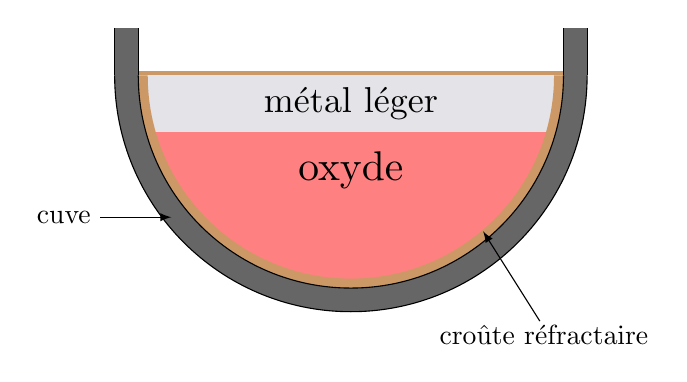
\begin{tikzpicture}[scale=0.60]
	%cuve
	%couche+croute
	\fill[red!50] (0.5,0) arc (180:360:4.5) -- cycle;
	%\fill[blue!10!gray!20] rectangle (9.5, 1);
	\fill[brown!80] rectangle (9.5,0.1);
	\fill[blue!10!gray!20] (0.5,0) rectangle (9.5, -1.2);
%	\fill[blue!10!gray!20] (2.5,-3.5) ..controls +(0.9,-1.05)and+(-0.9,-1.05) .. (7.5,-3.5) -- cycle ;
	\fill[black!60] (0,1) -- (0,0) arc (180:360:5) -- (10,1) -- (9.5,1) -- (9.5,0) arc (360:180:4.5) -- (0.5,1) -- cycle;
	\fill[brown!80] (0.5,0) arc (180:360:4.5) -- (9.3,0) arc (360:180:4.3) -- cycle;
	%cuve
	\draw (0,0) arc (180:360:5);
	\draw (0.5,0) arc (180:360:4.5);
	\draw (0,0) -- (0,1);
	\draw (0.5,0) -- (0.5,1);
	\draw (10,0) -- (10,1);
	\draw (9.5,0) -- (9.5,1);
	
	%\draw (5,0.5) node[ scale=1.3]{couche d'acier};
	\draw (5,-0.6) node[ scale=1.3]{métal léger};
	\draw (5,-2) node[ scale=1.5]{oxyde};
%	\draw (5,-3.8) node[ scale=1.3]{métal lourd};
	%		
	%		\draw[->,>=latex, red, line width = 2mm] (1.3, 0.5) to (0.1, 0.5);
	%		\draw[->,>=latex, red, line width = 2mm] (8.7, 0.5) to (9.9, 0.5);
	
	%FE
	%		\draw[black, dashed, thick] (3.2,0.2) circle (0.8);
	%\draw[black, dashed, thick] (9.3,0.5) circle (0.8);
	%		\draw[->,>=latex] (0.5, 0.8) to (4, 2);
	%		\draw[->,>=latex] (9.3, 0.8) to (6, 2);
	%		\draw (5,2.3) node[ scale=1.3]{Focusing Effect};
	
	%cuve
	\draw[->,>=latex] (-0.3, -3) to (1.2, -3);
	\draw (-0.3, -3) node[ scale=1, left]{cuve};
	
	%croute
	
		\draw[->,>=latex] (9, -5.2) to (7.8, -3.3);
%\draw (1, -4.2) -- (-0.3, -4.2);
\draw (11.5, -5.5) node[ scale=1, left]{croûte réfractaire};
	
	%echange
	%\draw[->,>=latex,line width = 0.8mm] (3.2, -0.6) to (3.2, -3.8);
	
	
	%		\draw[->,>=latex,line width = 0.5mm] (2.8, 0.8) to (2.8, -1.2);
	%		\draw (2.2,0.7) node[ scale=1]{(Fe)};
	%		\draw[->,>=latex,line width = 0.5mm](3.5, -1.2) to (3.5, 0.8);
	%		\draw (4.2,-1) node[ scale=1]{(U,Zr)};
	%\draw (2,0.5) node[ scale=1]{(Fe)};
	%\draw[->,>=latex,line width = 0.5mm](2.7, -1.2) to (2.7, 0.8);
	%\draw (3.4,-1) node[ scale=1]{(U,Zr)};
	%\draw[blue, very thick] (7.3, 0.1) -- (7.3, 1);
	%\draw[blue, thick] (7.2, 0.1) -- (7.4, 0.1);
	%\draw[blue, thick] (7.2, 1) -- (7.4, 1);
	%\draw (7.3, 0.5) node[ scale=1.3, right, blue]{$H$};
	\end{tikzpicture}
	\caption{Seconde configuration}
	\label{fig:confmetalleger}
\end{subfigure}
\caption{Présentation des différents régimes de stratification possibles}
\end{figure}
L'objectif de la rétention en cuve est alors de maintenir ce bain jusqu’à sa solidification, le refroidissement est assuré par de l'eau dans le puits de cuve et par rayonnement sur la face supérieur de la couche d'acier. Cependant la couche supérieure d'acier étant très conductrice et ayant un contact direct avec la cuve sur une surface très faible (la couche d'acier est haute de quelques dizaines de centimètres), la densité de flux transmise est très importante. Cet effet est appelé \textit{"focusing effect"} et représente la principale menace pour l'intégrité de la cuve.
%\subsubsection{Modélisation du régime transitoire}
Des études plus récentes ont montré que l'épaisseur de la couche d'acier pouvait être plus fine en régime transitoire qu'en régime stationnaire \cite{le_tellier_transient_2015}, diminuant ainsi la surface de contact et aggravant le \textit{"focusing effect"}, c'est pourquoi une modélisation en régime transitoire est désormais privilégiée. Lors du transitoire des phénomènes d'inversion de phase sont observés, une partie du métal de la phase légère s'alourdit sous l'effet d'un transfert de masse et des gouttes tombent, puis sous l'effet d'un même transfert de masse la phase lourde remonte. On observe alors trois couches : une couche d'oxyde, une de métal léger localisée au dessus de la couche d'oxyde et une couche de métal lourd en fond de cuve. Finalement, le schéma associé à l'étude du comportement d'un bain de corium en fond de cuve est présenté en figure \ref{fig:ivrschema}.
\begin{figure}[H]
	\centering
	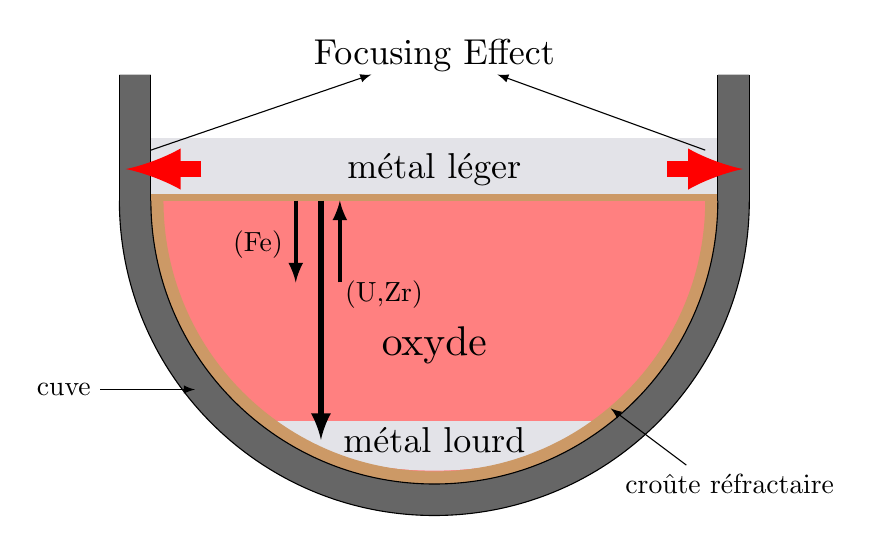
\begin{tikzpicture}[scale=0.80]
	

	
	%couche+croute
	\fill[red!50] (0.5,0) arc (180:360:4.5) -- cycle;
	\fill[blue!10!gray!20] (0.5,0) rectangle (9.5, 1);
	
	\fill[brown!80](0.5,0) rectangle (9.5,0.1);
	%\fill[blue!10!gray!20] (0.5,0) rectangle (9.5, -1.2);
	\fill[blue!10!gray!20] (2.5,-3.5) ..controls +(0.9,-1.05)and+(-0.9,-1.05) .. (7.5,-3.5) -- cycle ;
	\fill[brown!80] (0.5,0) arc (180:360:4.5) -- (9.3,0) arc (360:180:4.3) -- cycle;
	%cuve
	\fill[black!60] (0,2) -- (0,0) arc (180:360:5) -- (10,2) -- (9.5,2) -- (9.5,0) arc (360:180:4.5) -- (0.5,2) -- cycle;
	%cuve
	\draw (0,0) arc (180:360:5);
	\draw (0.5,0) arc (180:360:4.5);
	\draw (0,0) -- (0,2);
	\draw (0.5,0) -- (0.5,2);
	\draw (10,0) -- (10,2);
	\draw (9.5,0) -- (9.5,2);
	
	\draw (5,0.5) node[ scale=1.3]{métal léger};
	\draw (5,-2.3) node[ scale=1.5]{oxyde};
	\draw (5,-3.8) node[ scale=1.3]{métal lourd};
	%\draw (6,-0.6) node[ scale=1.3]{métal léger};
	
	\draw[->,>=latex, red, line width = 2mm] (1.3, 0.5) to (0.1, 0.5);
	\draw[->,>=latex, red, line width = 2mm] (8.7, 0.5) to (9.9, 0.5);
	
	%FE
	%\draw[black, dashed, thick] (3.2,-1) circle (0.5);
	%\draw[black, dashed, thick] (9.3,0.5) circle (0.8);
	\draw[->,>=latex] (0.5, 0.8) to (4, 2);
	\draw[->,>=latex] (9.3, 0.8) to (6, 2);
	\draw (5,2.3) node[ scale=1.3]{Focusing Effect};
	
	%cuve
	\draw[->,>=latex] (-0.3, -3) to (1.2, -3);
	\draw (-0.3, -3) node[ scale=1, left]{cuve};
	
	%croute
	
	\draw[->,>=latex] (9, -4.2) to (7.8, -3.3);
	%\draw (1, -4.2) -- (-0.3, -4.2);
	\draw (11.5, -4.5) node[ scale=1, left]{croûte réfractaire};
	
	%echange
	\draw[->,>=latex,line width = 0.8mm] (3.2, 0) to (3.2, -3.8);
	
	
	\draw[->,>=latex,line width = 0.5mm] (2.8, -0) to (2.8, -1.3);
	\draw (2.2,-0.7) node[ scale=1]{(Fe)};
	\draw[->,>=latex,line width = 0.5mm](3.5, -1.3) to (3.5, -0);
	\draw (4.2,-1.5) node[ scale=1]{(U,Zr)};
	%\draw (2,0.5) node[ scale=1]{(Fe)};
	%\draw[->,>=latex,line width = 0.5mm](2.7, -1.2) to (2.7, 0.8);
	%\draw (3.4,-1) node[ scale=1]{(U,Zr)};
	%\draw[blue, very thick] (7.3, 0.1) -- (7.3, 1);
	%\draw[blue, thick] (7.2, 0.1) -- (7.4, 0.1);
	%\draw[blue, thick] (7.2, 1) -- (7.4, 1);
	%\draw (7.3, 0.5) node[ scale=1.3, right, blue]{$H$};
	\end{tikzpicture}
	\caption[]{Schéma du comportement du corium en fond de cuve en régime transitoire}
	\label{fig:ivrschema}
\end{figure}
La couche de métal lourd se forme à partir d'un transfert de masse à l'interface des phases oxyde et métal léger créant des gouttes de métal lourd se relocalisant en fond de cuve. Il existe peu de données expérimentales sur le comportement du corium en cuve du fait de la difficulté de réalisation expérimentale liée aux conditions de température supérieures à 2000K. MASCA RCW \cite{tsurikov_main_nodate} est une des rares expériences sur la stratification ayant mis en jeu une quantité suffisante de matière pour retranscrire la cinétique d'un accident. Cet essai utilise du corium prototypique (non radioactif) chauffé par induction. Lors de l'essai 45kg de corium ont été mis en contact avec 4kg d'acier, cette configuration permet d'obtenir un régime stationnaire caractérisé par la présence d'une phase métallique lourde (figure \ref{fig:confmetallourd}). L'essai a été arrêté avant que le système n'atteigne le régime stationnaire. Une photo de la découpe du lingot est présentée en figure \ref{fig:masca}. On y observe la présence de gouttes formées par des instabilités de Rayleigh-Taylor issus de la couche métallique légère. Aucune expérience similaire n'a permis d'observer le phénomène de remontée de la phase métallique lourde.

 \begin{figure}[H]
	\centering
	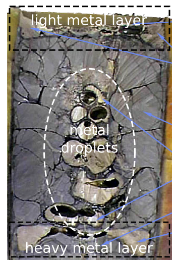
\includegraphics[width=0.3\linewidth]{figure/MASCA_RCW.png}
	\caption[Résultat MASCA-RCW 100]{Résultat MASCA-RCW, d'après \cite{tellier_interfaces_2019}}
	\label{fig:masca}
\end{figure}


\section{Objectif du stage}
Le LMAG s'intéresse à la modélisation du transfert de masse mis en jeu lors de transitoires de stratification pour mieux comprendre le comportement d'un bain de corium en fond de cuve. Pour permettre une meilleure compréhension des phénomènes le laboratoire développe deux types d'outils. Le premier est un modèle intégral implémenté dans la plateforme logicielle PROCOR \cite{le_tellier_phenomenological_2015}, développée au LMAG et utilisé par les industriels pour l’étude de la propagation du corium. Simultanément, des recherches sont également menées pour obtenir une modélisation à des échelles CFD (\textit{Computional Fluid Dynamic}) plus fines. Dans ce cadre une partie du laboratoire s'intéresse à la modélisation champ de phase pour considérer le transfert de masse aux interfaces lors de transitoires de stratification.\\ Les recherches ont commencé avec la thèse de C. Cardon \cite{cardon_modelisation_2016} sur la diffusion d'espèce dans un système multicomposant diphasique et le paramétrage associé en lien avec les bases thermodynamiques. Dans le cadre du contrat post-doctoral de R. Zanella l'étude de la faisabilité d'un modèle pseudo-binaire couplé à l'hydrodynamique a pu être menée. L'objectif était de reproduire qualitativement l'expérience MASCA-RCW \cites{zanella_two-_2020}{zanella_three-dimensional_2021} en utilisant un code pseudo-spectral. Finalement dans la thèse de M.A. Rasolofomanana \cite{rasolofomanana_modelisation_nodate} le couplage entre un système multicomposant multiphasique et l'hydrodynamique est réalisé au travers de l'implémentation de l'équation de Cahn-Hilliard généralisée dans TrioCFD  \cite{angeli_overview_2015} (code CFD Open-source CEA).\\
L'objectif général de ce stage est de tester ce modèle et son implémentation et de fournir des premiers éléments de validation. Pour ce faire, on s'intéressera en premier lieu au cas d'une goutte isolée dans une phase continue au travers d'une expérience de la littérature \cite{rao_influence_2015}. Cette expérience montre l’influence du transfert de masse sur la trajectoire d’une goutte multicomposant. En l'état du code, les simulations peuvent difficilement être quantitative, dans notre cas, on se limitera à une étude paramétrique et à des éléments de comparaison qualitatifs. Ensuite, de manière complémentaire, des simulations ont été réalisées afin d'évaluer la capacité de ce modèle à reproduire différents régimes de gouttes. Pour finir, en revenant vers l'objectif général associé à la simulation d'un bain de corium, une simulation de l'inversion de stratification d'un bain stratifié a été réalisée. \\
Le deuxième chapitre se concentre sur les notions théoriques liées à la méthode champ de phase et sur les choix de paramétrage du modèle. Le troisième chapitre présente les résultats pour une goutte isolée et non déformée soumise à du transfert de masse et la comparaison avec \cite{rao_influence_2015}. Dans le chapitre 4 certains régimes de déformation d'une goutte non soumise à du transfert de masse sont retrouvés. Le cinquième chapitre présente des simulations proche du cas d'intérêt du corium, avec des calculs d'instabilités de Rayleigh-Taylor entraînant l'inversion de stratification dans un bain. Finalement, au terme de ce rapport, une courte conclusion ainsi que des perspectives sont apportées.

% Le développement de ce type de code nécessite une compréhension des phénomènes à des échelles plus fine. Sans données expérimentales, la modélisation à l'échelle CFD (\textit{Computional Fluid Dynamic}).
%
%
%L'objectif du stage est de réaliser une validation qualitative d'un modèle CFD (\textit{Computional Fluid Dynamic}) implémenté dans TrioCFD, code Open-Source du CEA, par M.A Rasolofomanana lors de sa thèse \cite{rasolofomanana_modelisation_nodate}. Ce modèle est une généralisation de la méthode champ de phase pour un système multicomposant. Cette implémentation fait suite aux thèses de Clément Cardon \cite{cardon_modelisation_2016} et de Vaishnvi Tiwari \cite{tiwari_consistent_2019} sur la modélisation par la méthode de champ de phase pour un système multicomposant. L'expérience reproduite est présentée dans \cite{rao_influence_2015}, on y trouve une goutte qui sous l'effet d'un transfert de masse va subir une inversion de densité. Cette validation nécessite une paramétrisation cohérente du système pour obtenir des simulations consistante vis-a-vis d'un système binaire et du comportement thermodynamique. Le développement de ce type de code CFD a pour but de permettre la vérification et l'amélioration des lois de fermetures présente dans des codes intégraux, comme par exemple PROCOR développé au laboratoire.